\section{ARCADIA MD1}
ARCADIA (Advanced Readout CMOS Architectures with Depleted Integrated sensor Arrays)\cite{ARCADIA-Pancheri}\cite{ARCADIA-Pancheri2} and SEED (Sensor with Embedded Electronic Development) are collaborations involved in the development of MAPS sensors based on the CMOS technology and both having LFoundry as industrial partner.
Many concept and performances studies have been carried out with simulations and small-scale test structure by SEED, before ARCADIA, applying the experience developed with SEED to a full chip prototype, the MD1.  
MATISSE is an example of small-scale prototypes produced for testing: it is made by 24$\times$24 pixels organized in 4 columns; each pixel has an analog output, which allows for energy loss measurements, and a shutter snapshot readout with a speed that can reach \SI{5}{MHz}. 

The ARCADIA target is the development of a novel CMOS sensor platform allowing for fully depleted active sensors with thickness in the range \SIrange{50}{500}{\um}. A small charge collecting electrode to achieve a good signal to noise ratio, a high time resolution (the lower bound is set at O(\si{\us}) but more advanced solutions are investigating for a O(\SI{10}{ns})) and a scalable readout architecture with low power consumption are the main requirement imposed by ARCADIA; the Main Demonstrator 1, has been submitted in 2020, and its characteristic are shown in table \ref{tab:ARCADIA_MD1}.
A second main demonstrator (ARCADIA-MD2) has been submitted in Summer 2021, featuring a similar design of MD1, but is expected to be faster and to have a lower power consumption thanks to a logic and buffering optimization. 

\begin{table}
    \begin{center}
    \begin{tabular}{| c |c |}
    \hline
    Parameter & Value\\
    \hline
    \hline
    Matrix size & 1.28$\times$1.28 \si{cm\squared}\\
    Pixel size & 25$\times$25 \si{\um\squared}\\
    Depth &  48/100/200\si{\um}\\
    Electrode size & 9$\times$9\si{\um\squared}\\
    Power consumption & $\sim$ 10\si{mW/cm\squared}\\ 
    Output signal & digital \\
    \hline
    \end{tabular}
    \caption{}
    \label{tab:ARCADIA_MD1}
    \end{center}
\end{table}

\subsection{The sensor and the front end}
    \begin{figure}[h!]
        \centering
        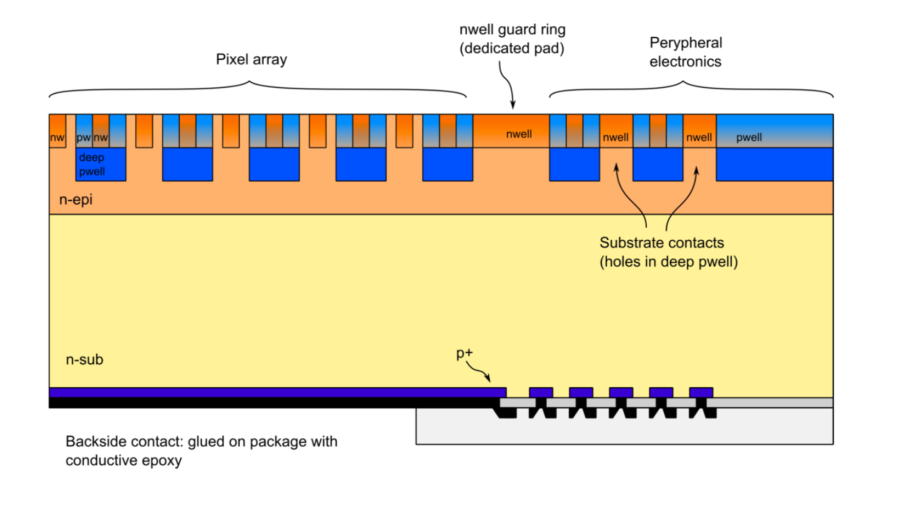
\includegraphics[width=.8\linewidth]{figures/ARCADIA/sensor.png}
        \caption{Cross section of the ARCADIA MD1 sensor}
        \label{fig:ARCADIA_substrate}
    \end{figure}
    ARCADIA-MD1 is an LFoundry chip fabricated in \SI{110}{nm} CMOS technology.%\ref{articolo_ fully depl}.
    The sensor (fig.\ref{fig:ARCADIA_substrate}) is made by a $p$ substrate and an $n$ doped diode within a $n$ epitaxial layer; a custom patterned backside has been developed in collaboration with LFoundry to introduce junction at the bottom surface which allows a full depletion. 
    A deep p-well enclosure has been used to shield the n-well contained in the electronics circuit and deny competing in charge collection; considering the isolation the resulting area available for the analog circuit is \SI{223}{\um\squared}.

    Up to now the sensor has been implemented in three different variant: \SI{48}{\um}, \SI{100}{\um} and \SI{200}{\um} thick, each with the same FE and readout logic but requiring a different biasing (always higher than \SI{10}{V}). 
    In figure \ref{fig:ARCADIA_E} is shown a TCAD simulation, which includes two pixels and a guard ring, of the electric-field line within the sensor; being part of DMAPS and being operated in fully depletion, the charge is fastly collected by drift along the electric field lines. 
    \begin{figure}[h!]
        \centering
        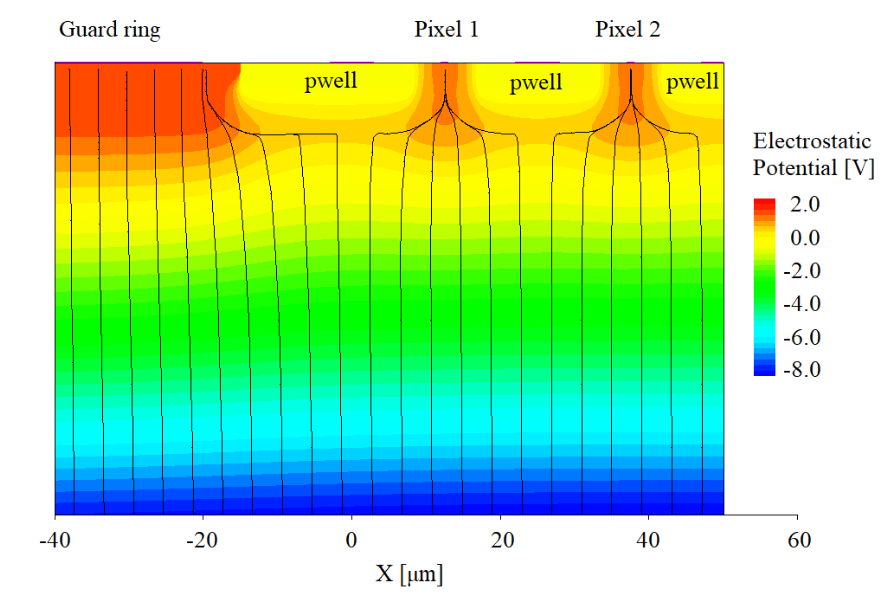
\includegraphics[width=.8\linewidth]{figures/ARCADIA/ARCADIA_TCAD.png}
        \caption{TCAD simulation of the electric field in the surface region of the sensor.}
        \label{fig:ARCADIA_E}
    \end{figure}

        There are three types of configuration registers which are used to configure the matrix: 
        \begin{itemize}
            \item the Pixel Configuration Register (PCR), which is a 2-bits word used for enabling respectively the masking and injection functionalities. Each bit is made by a latch which occupy \SI{14.6}{\um\squared} out of the per-pixel area available, \SI{223}{\um\squared} then it is clear that there is not much extra space for any more configuration bits. The on-pixel PCR circuit is shown in figure \ref{fig:pixel_cfg}.
            \item the Internal Configuration Register (ICR), which are used for the comunication with the FPGA, for example to send a pulse, reset or configure the whole matrix.
            \item the Global Configuration Registers (GCR), which are used to set the configuration of the FE parameters are similar to the one of the TJ-Monopix1 circuit, and they are (partially) listed in table \ref{tab:FE_ARCADIA-parameters}.
        \end{itemize}
        Their bias with the one of the sensors are supplied by padframes (a top, a bottom and a side one) placed aside the matrix, which also provide the clock, the reset, the test pulse for the injection circuit and the comunication signals.
        The timestamp clock, which defines the timestamp granularity, is not internally generated but it is obtained from an external clock of \SI{320}{MHz} with a clock divider; a 4-bit GCR is used set the base-2 logarithm of the dividing ratio, such as the timestamp clock frequency is:
        \begin{equation}
            f_{timestamp}\, =\, \frac{\SI{320}{MHz}}{2^{GCR}}
        \end{equation}
        and then varies in range \SI{320}{MHz} and \SI{20}{MHz}.\\
        \begin{figure}[h!]
            \centering
            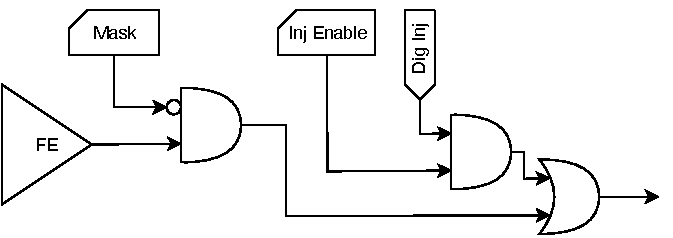
\includegraphics[width=.7\linewidth]{figures/ARCADIA/pixel_cfg.pdf}
            \caption{Logic used for each pixel to implement the injection and the masking.}
            \label{fig:pixel_cfg}
        \end{figure}    
        %Inoltre ci sono altre differenze, il bulk driven è più sensibile alle cadute di tensione sul ground (che ahimè è esattamente ciò che accade nei dimostratori che abbiamo ora, a causa dell'anomalo consumo di corrente dal digitale, altro baco che abbiamo corretto nella terza sottomissione).
        %Anche i livelli di tensione nei nodi interni dei due front-end differiscono e il meccanismo di clipping che funzionava per l'Alpide non è applicabile al bulk driven. Di conseguenza abbiamo un bias in più (ICLIP) nel secondo flavour per controllare il clipping. Nell'Alpide il clipping c'è, ma l'architettura usata permette di non aver bisogno di un bias esterno, anche se in una versione di Alpide di ALICE hanno scelto di controllare comunque la corrente di clip esternamente, per una maggiore flessibilità. Infine alcuni bias che hanno lo stesso nome nei due flavour, perché svolgono la stessa funzione, differiscono nel valore di configurazione didefault.
        \begin{table}
            \begin{center}
            \begin{tabular}{|c | c |}
            \hline
            Parameter & Meaning \\
            \hline
            \hline
            CLK\_DIVIDER & log$_2$ number to divide the input clock  \\
            VINREF & provides the current to restore the input node i\\
            VCASN & sets the threshold\\
            IBIAS & sets the baseline\\
            IFB & current in the feedback branch \\
            ID & discriminator current\\
            ICLIP & baseline \\
            \hline
            \end{tabular}
            \caption{FE MD1 parameters which must be setted through the DAQ.}
            \label{tab:FE_ARCADIA-parameters}
            \end{center}
        \end{table}

        MD1 chips have been submitted in two different front end options: they are commonly called ALPIDE-like and bulk-driven.  
        The differences between them are in the FE circuit and in the biasing current of the registers, while the underlying readout is the same.
        The main difference is in the amplification stage, while in the ALPIDE-like flavor the amplification is implemented as explained in section \ref{sec:ALPIDE-like}, in the bulk-driven flavor the gain is adjusted by the ratio of two transconduttances. Consequently, some of the biasing registers, whose current is settable externally by the DAQ, have different default values and they might not be available at all in one of the flavor.
        An example is the ICLIP register, which is available only in the bulk driven flavor despite the transistor to which refers is implemented in both the flavor; its function is similar to the \emph{curfeed} capacitor in figure \ref{fig:Monopix1_FE_circuit}(a), which controls the current in the input branch of the FE and also influences the value of the baseline at the discriminator input. 


\subsection{Readout logic and data structure}
    \begin{figure}[h!]
        \centering
        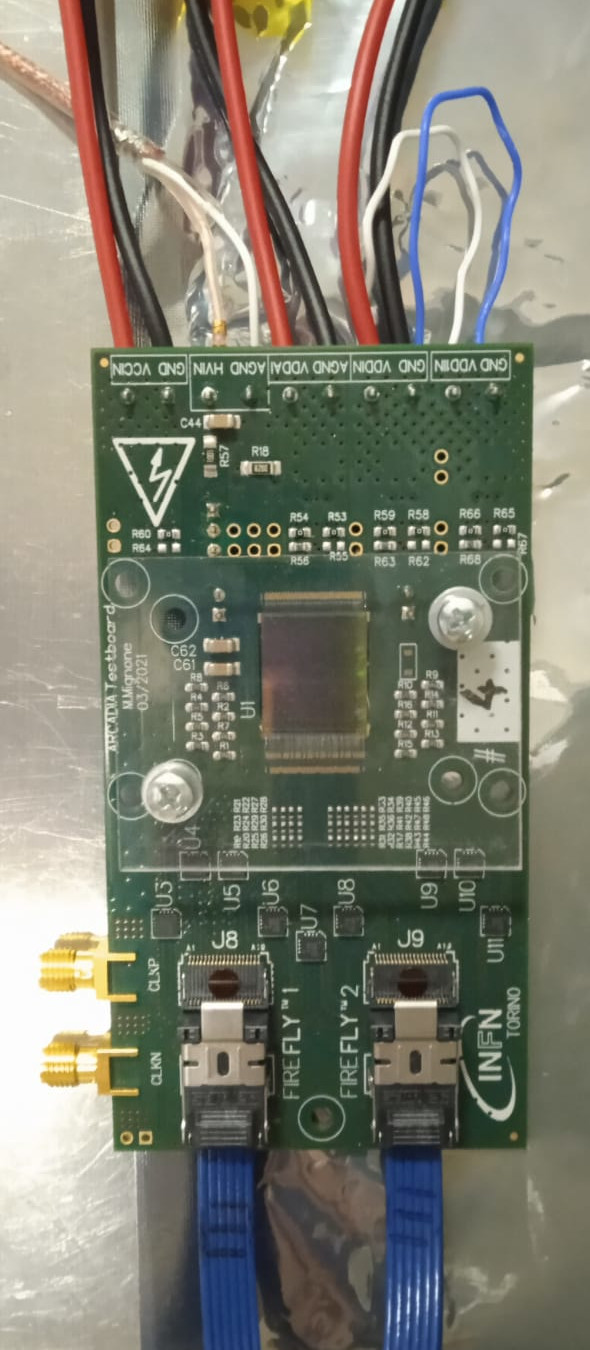
\includegraphics[width=.3\linewidth, angle =90 ]{figures/ARCADIA/arcadia_chip_front.jpeg}\\
        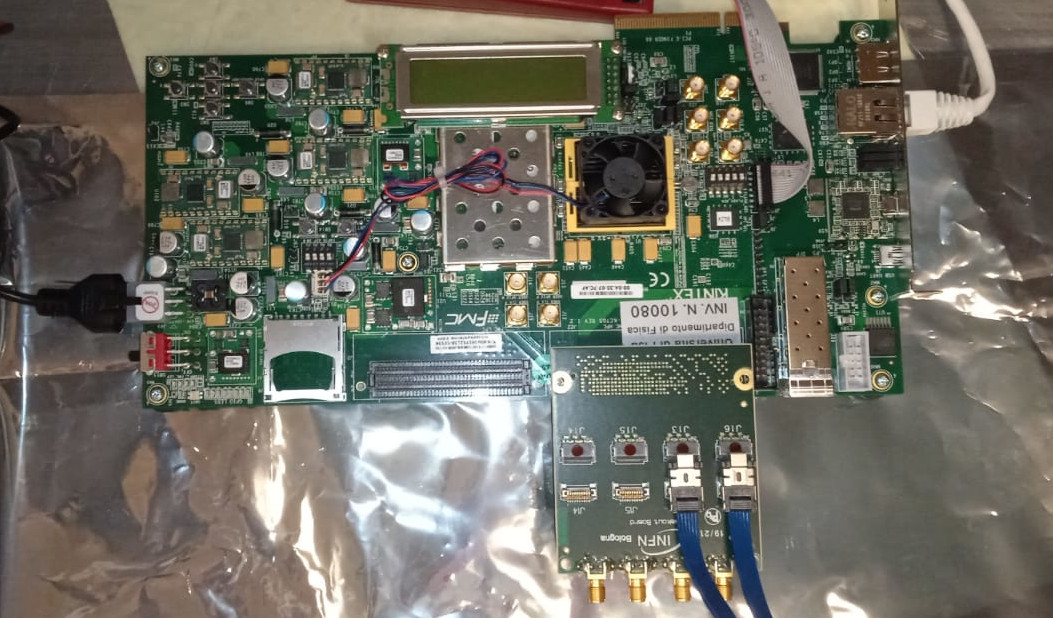
\includegraphics[width=.7\linewidth]{figures/ARCADIA/arcadia_FPGA.jpeg}
        \caption{(a) Board hosting the MD1 chip. (b) FPGA and breakout board. The chip and breakout boards must be connected with the blue cables}
        \label{fig:foto_setup}
    \end{figure}
    One of the main ambition of the MD1 is to achieve the lowest possible power consumption, hopefully less than \SI{20}{mW/cm\squared}; this is important for applications in the field of space experiment, where the power consumption and the cooling are a major issue. 
    In order to fulfill that requirement, the matrix is clockless and the readout is triggerless; moreover the chip can be operated both in the high rate mode and low rate by enabling on if only one or all serializers, placed at the periphery of the matrix. In addition, to save as much area as possible, buffers have not been included on the matrix, at the expense of the maximum hit rate sustainable. The readout then is completely data push and when a hit is received immediately starts the readout mechanism to transmit it off chip.
    The board hosting the chip is connected with a breakout board, which is connected to the FPGA; a data packet sent to the EoS, is then encoded and transmitted to the FPGA using a \SI{320}{MHz} DDR serializers and then transmitted by ethernet to the PC.
    %Sections with own 320MHz DDR Output link. The sections will have to have their own output link, in order to ease future up-scaling.-> lo dicono come requirement
    A photo of the experimental setup is shown in figure \ref{fig:foto_setup}.

        \begin{figure}[h!]
            \centering
            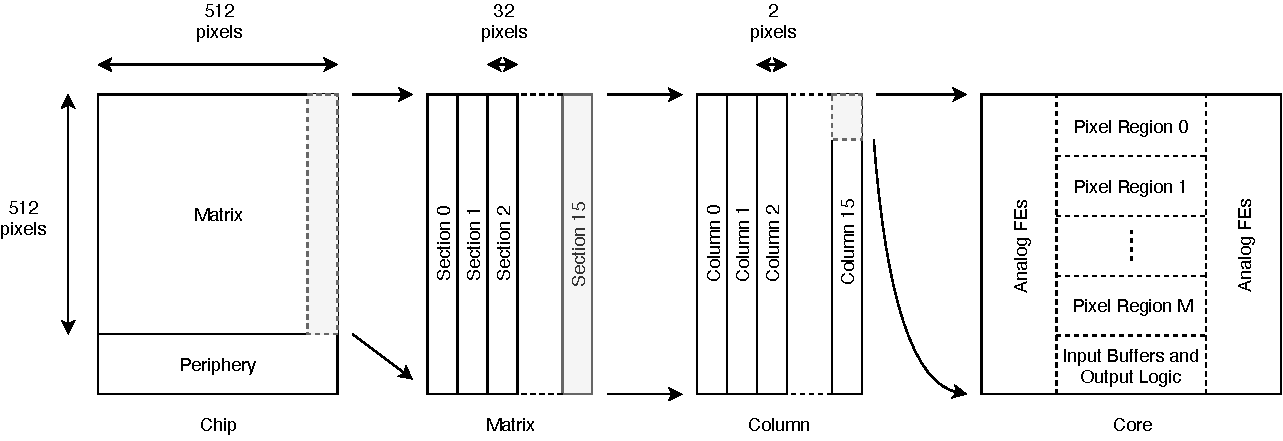
\includegraphics[width=.98\linewidth]{figures/ARCADIA/hierarchy.pdf}
            \caption{Hierarchy of the matrix division}
            \label{fig:hierarchy}
        \end{figure}
        The chip structure is meant to optimize the power consumption and the scalability for future up-scaling retaining high rate operation; in particular it is divided into a physical and logical hierarchy, which also reflects in the way the data packets are built (tab.\ref{tab:data_packet}).
        First of all, the 512 columns are split in 16 sections each one containing 512$\times$32 pixels and having its own biasing lines and serializers at the matrix periphery. 
        Each section is is divided 512$\times$2 double-column mirrored, which just as in TJ-Monopix1, share the same readout buses placed between them and having analog logic on the sides.        
        The rows, then, are divided in group of 32, resulting in core with 32$\times$2 pixels. Finally each core is sub-divided in regions, each one containing 4$\times$2 pixels. 
        \begin{table}
            \begin{center}
            \begin{tabular}{|c |c |}
            \hline
            Bits & Meaning  \\
            \hline
            \hline
            31:24 & timestamp\\
            23:20 & section index\\
            19:16 & column index\\
            15:9 & pixel region\\
            8:0 & hitmap\\
            \hline
            \end{tabular}
            \caption{Data packet structure implemented by the MD1 readout logic.}
            \label{tab:data_packet}
            \end{center}
        \end{table}

        The readout has been designed with the constraints of being capable of handling a rate of \SI{100}{MHz/cm\squared}, and it has been optimized to minimize the amount of logic and to have a high bandwidth of transmission of the data to the periphery. For this reason not all pixels have been provided of the readout logic.
        In particular, each pixel region can either be Master or Slave, depending on if has or has not the readout capability. 
        The Master's data packets are therefore composed of two parts: the hitmap of the Master itself and the one of Slave. 
        Moreover, the pioneer idea of ARCADIA-MD1, which has as finally goal the test of a readout capable of transmit cluster data in as few data packets as possible, is the possibility of the Master to decide what Slave (top or bottom) to read; the information of what Slave has been selected is represented by a bit, often called \emph{hot bit}, in the data-packet.
        Every pixel has an associated status register, that essentially is a flip flop (FF), which is set to 1 when the pixel stores a hit; an OR of the FF within the Master or the Slave region generates an active flag which is used to require a readout by the EoS.  
        \begin{figure}[h!]
            \centering
            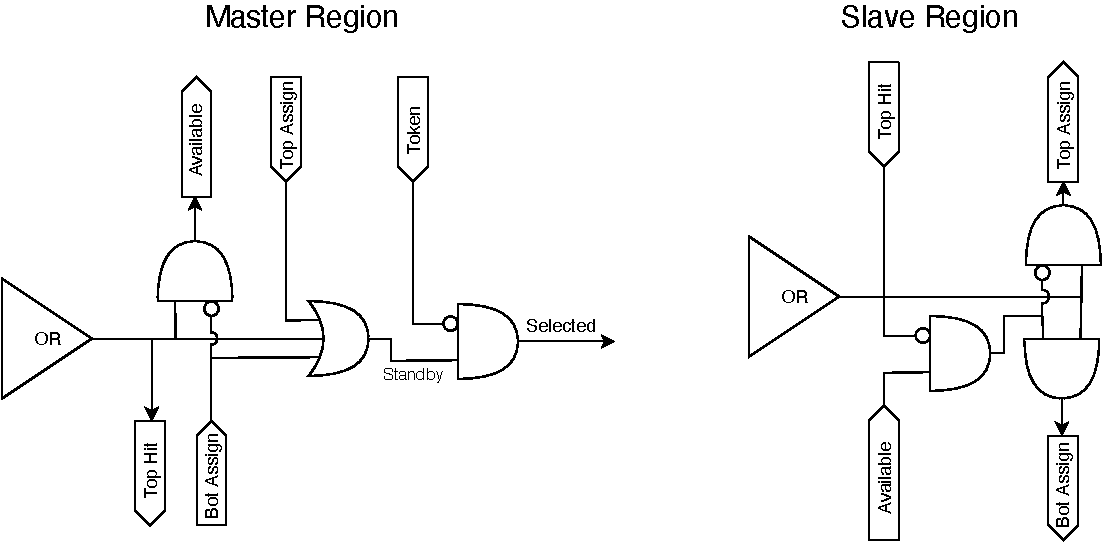
\includegraphics[width=.95\linewidth]{figures/ARCADIA/clustering_logic.pdf}
            \caption{Logic of the circuit to implement the online clustering and deciding if to assign the Slave to the top or bottom Master.}
            \label{fig:clustering_logic}
        \end{figure}
        In figure \ref{fig:clustering_logic} is shown the circuit with the logic of assignment of the Slave to the Master.
        

        Depending on the active flags of the neighbours Masters, the Slave hitmap is assigned to the one at the top or bottom. 
        %\red{The circuit which does that is shown in figure \ref{fig:clustering_logic}}. 
        If both the Masters have an active flag, the Slave is assigned to the top one. 
        \begin{figure}[h!]
            \centering
            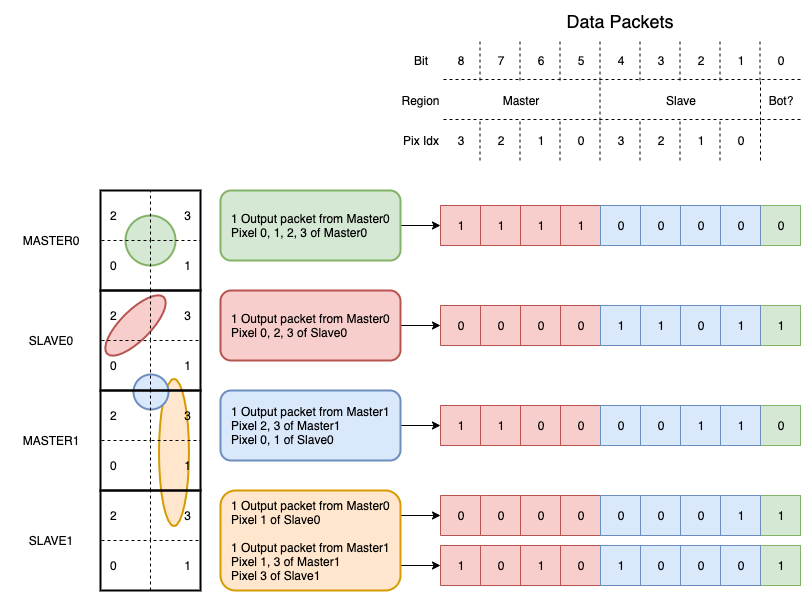
\includegraphics[width=.95\linewidth]{figures/ARCADIA/clustering.png}
            \caption{Different cluster structures and the data packet produced by them are shown in the example.}
            \label{fig:clustering}
        \end{figure}
        In the example in figure \ref{fig:clustering} two Master-Slave regions are considered: the hitmaps of the Master (red colored in the example) and Slave (blue colored) are joined together within a unique data packet and a bit (green colored) is used to specify the Slave. 

        The data packets are transmitted to the End of Section (EoS) with a priority chain similar to what happens in TJ-Monopix1. 
        If at least one Master set a high flag, a \textcolor{Cerulean}{Token} signal is generated and is assigned to the high priority Master in the column, together with a \textcolor{red}{Full} flag which is distributed to the active Masters in the whole column in order to deny more region to be accessed at the same time.
        The readout then propagates down the column from Master to Master, skipping the empty cores; the Master selected for the readout is the one with the flag high and with an input (from top) \textcolor{Cerulean}{Token} equal to 0. 
        In the example in figure \ref{fig:token_chain} the \textcolor{Cerulean}{Token} is propagated from the Pixel Region (PR) 10 to the PR 7. 
        In the three readout steps the red Masters are the ones selected for the readout, while the yellow are the ones which an active flag high; gray color is used for empty regions. When a specific Master has been selected, a \textcolor{Cerulean}{Read} signal is generated both to transmit the data to the EoS and also to generate a reset for the just read pixels.
        Once the pixels are reset, the Master's \textcolor{red}{Full} 
        and \textcolor{Cerulean}{Token} flags fall, and the following region which satisfies the two readout conditions explained above, becomes selected. 
        \begin{figure}[h!]
            \centering
            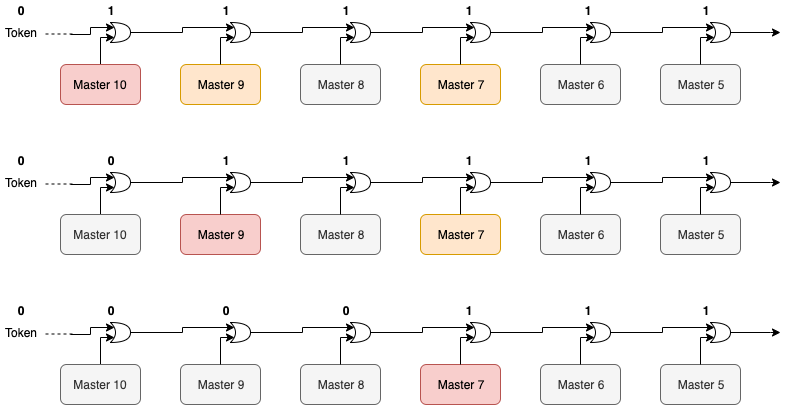
\includegraphics[width=.95\linewidth]{figures/ARCADIA/token_chain.png}
            \caption{Three steps in the readout sequence on the region-column: the Token is propagated from the Master 10, to Master 9 and then to Master 7, according to the priority chain readout.}
            \label{fig:token_chain}
        \end{figure}

    The performances of the readout has been studied with simulations by the designer of the chip. 
    Random hits events with cluster size of 4 pixels on average, with a Poissonian distribution in time and uniformly distributed on the matrix has been generated.
    They state that with particle hit rate of \SI{100}{MHz/cm\squared}, considering a portion of matrix of three section (512$\times$96), the efficiency results to be 98.7\%, while reducing the hit rate to \SI{80}{MHz/cm\squared} it is even higher achieving the 99.95\%. 
